\documentclass[]{book}
\usepackage{lmodern}
\usepackage{amssymb,amsmath}
\usepackage{ifxetex,ifluatex}
\usepackage{fixltx2e} % provides \textsubscript
\ifnum 0\ifxetex 1\fi\ifluatex 1\fi=0 % if pdftex
  \usepackage[T1]{fontenc}
  \usepackage[utf8]{inputenc}
\else % if luatex or xelatex
  \ifxetex
    \usepackage{mathspec}
  \else
    \usepackage{fontspec}
  \fi
  \defaultfontfeatures{Ligatures=TeX,Scale=MatchLowercase}
\fi
% use upquote if available, for straight quotes in verbatim environments
\IfFileExists{upquote.sty}{\usepackage{upquote}}{}
% use microtype if available
\IfFileExists{microtype.sty}{%
\usepackage{microtype}
\UseMicrotypeSet[protrusion]{basicmath} % disable protrusion for tt fonts
}{}
\usepackage{hyperref}
\hypersetup{unicode=true,
            pdftitle={Hurricane Analysis and Visulization Using R},
            pdfauthor={Romane Goldmuntz, Vy Tran, and Jianqiong Zhan},
            pdfborder={0 0 0},
            breaklinks=true}
\urlstyle{same}  % don't use monospace font for urls
\usepackage{natbib}
\bibliographystyle{apalike}
\usepackage{color}
\usepackage{fancyvrb}
\newcommand{\VerbBar}{|}
\newcommand{\VERB}{\Verb[commandchars=\\\{\}]}
\DefineVerbatimEnvironment{Highlighting}{Verbatim}{commandchars=\\\{\}}
% Add ',fontsize=\small' for more characters per line
\usepackage{framed}
\definecolor{shadecolor}{RGB}{248,248,248}
\newenvironment{Shaded}{\begin{snugshade}}{\end{snugshade}}
\newcommand{\AlertTok}[1]{\textcolor[rgb]{0.94,0.16,0.16}{#1}}
\newcommand{\AnnotationTok}[1]{\textcolor[rgb]{0.56,0.35,0.01}{\textbf{\textit{#1}}}}
\newcommand{\AttributeTok}[1]{\textcolor[rgb]{0.77,0.63,0.00}{#1}}
\newcommand{\BaseNTok}[1]{\textcolor[rgb]{0.00,0.00,0.81}{#1}}
\newcommand{\BuiltInTok}[1]{#1}
\newcommand{\CharTok}[1]{\textcolor[rgb]{0.31,0.60,0.02}{#1}}
\newcommand{\CommentTok}[1]{\textcolor[rgb]{0.56,0.35,0.01}{\textit{#1}}}
\newcommand{\CommentVarTok}[1]{\textcolor[rgb]{0.56,0.35,0.01}{\textbf{\textit{#1}}}}
\newcommand{\ConstantTok}[1]{\textcolor[rgb]{0.00,0.00,0.00}{#1}}
\newcommand{\ControlFlowTok}[1]{\textcolor[rgb]{0.13,0.29,0.53}{\textbf{#1}}}
\newcommand{\DataTypeTok}[1]{\textcolor[rgb]{0.13,0.29,0.53}{#1}}
\newcommand{\DecValTok}[1]{\textcolor[rgb]{0.00,0.00,0.81}{#1}}
\newcommand{\DocumentationTok}[1]{\textcolor[rgb]{0.56,0.35,0.01}{\textbf{\textit{#1}}}}
\newcommand{\ErrorTok}[1]{\textcolor[rgb]{0.64,0.00,0.00}{\textbf{#1}}}
\newcommand{\ExtensionTok}[1]{#1}
\newcommand{\FloatTok}[1]{\textcolor[rgb]{0.00,0.00,0.81}{#1}}
\newcommand{\FunctionTok}[1]{\textcolor[rgb]{0.00,0.00,0.00}{#1}}
\newcommand{\ImportTok}[1]{#1}
\newcommand{\InformationTok}[1]{\textcolor[rgb]{0.56,0.35,0.01}{\textbf{\textit{#1}}}}
\newcommand{\KeywordTok}[1]{\textcolor[rgb]{0.13,0.29,0.53}{\textbf{#1}}}
\newcommand{\NormalTok}[1]{#1}
\newcommand{\OperatorTok}[1]{\textcolor[rgb]{0.81,0.36,0.00}{\textbf{#1}}}
\newcommand{\OtherTok}[1]{\textcolor[rgb]{0.56,0.35,0.01}{#1}}
\newcommand{\PreprocessorTok}[1]{\textcolor[rgb]{0.56,0.35,0.01}{\textit{#1}}}
\newcommand{\RegionMarkerTok}[1]{#1}
\newcommand{\SpecialCharTok}[1]{\textcolor[rgb]{0.00,0.00,0.00}{#1}}
\newcommand{\SpecialStringTok}[1]{\textcolor[rgb]{0.31,0.60,0.02}{#1}}
\newcommand{\StringTok}[1]{\textcolor[rgb]{0.31,0.60,0.02}{#1}}
\newcommand{\VariableTok}[1]{\textcolor[rgb]{0.00,0.00,0.00}{#1}}
\newcommand{\VerbatimStringTok}[1]{\textcolor[rgb]{0.31,0.60,0.02}{#1}}
\newcommand{\WarningTok}[1]{\textcolor[rgb]{0.56,0.35,0.01}{\textbf{\textit{#1}}}}
\usepackage{longtable,booktabs}
\usepackage{graphicx}
% grffile has become a legacy package: https://ctan.org/pkg/grffile
\IfFileExists{grffile.sty}{%
\usepackage{grffile}
}{}
\makeatletter
\def\maxwidth{\ifdim\Gin@nat@width>\linewidth\linewidth\else\Gin@nat@width\fi}
\def\maxheight{\ifdim\Gin@nat@height>\textheight\textheight\else\Gin@nat@height\fi}
\makeatother
% Scale images if necessary, so that they will not overflow the page
% margins by default, and it is still possible to overwrite the defaults
% using explicit options in \includegraphics[width, height, ...]{}
\setkeys{Gin}{width=\maxwidth,height=\maxheight,keepaspectratio}
\IfFileExists{parskip.sty}{%
\usepackage{parskip}
}{% else
\setlength{\parindent}{0pt}
\setlength{\parskip}{6pt plus 2pt minus 1pt}
}
\setlength{\emergencystretch}{3em}  % prevent overfull lines
\providecommand{\tightlist}{%
  \setlength{\itemsep}{0pt}\setlength{\parskip}{0pt}}
\setcounter{secnumdepth}{5}
% Redefines (sub)paragraphs to behave more like sections
\ifx\paragraph\undefined\else
\let\oldparagraph\paragraph
\renewcommand{\paragraph}[1]{\oldparagraph{#1}\mbox{}}
\fi
\ifx\subparagraph\undefined\else
\let\oldsubparagraph\subparagraph
\renewcommand{\subparagraph}[1]{\oldsubparagraph{#1}\mbox{}}
\fi

%%% Use protect on footnotes to avoid problems with footnotes in titles
\let\rmarkdownfootnote\footnote%
\def\footnote{\protect\rmarkdownfootnote}

%%% Change title format to be more compact
\usepackage{titling}

% Create subtitle command for use in maketitle
\providecommand{\subtitle}[1]{
  \posttitle{
    \begin{center}\large#1\end{center}
    }
}

\setlength{\droptitle}{-2em}

  \title{Hurricane Analysis and Visulization Using R}
    \pretitle{\vspace{\droptitle}\centering\huge}
  \posttitle{\par}
    \author{Romane Goldmuntz, Vy Tran, and Jianqiong Zhan}
    \preauthor{\centering\large\emph}
  \postauthor{\par}
      \predate{\centering\large\emph}
  \postdate{\par}
    \date{2019-12-12}

\usepackage{booktabs}
\usepackage{amsthm}
\makeatletter
\def\thm@space@setup{%
  \thm@preskip=8pt plus 2pt minus 4pt
  \thm@postskip=\thm@preskip
}
\makeatother

\begin{document}
\maketitle

{
\setcounter{tocdepth}{1}
\tableofcontents
}
\hypertarget{intro}{%
\chapter{Introduction}\label{intro}}

\begin{figure}
\centering
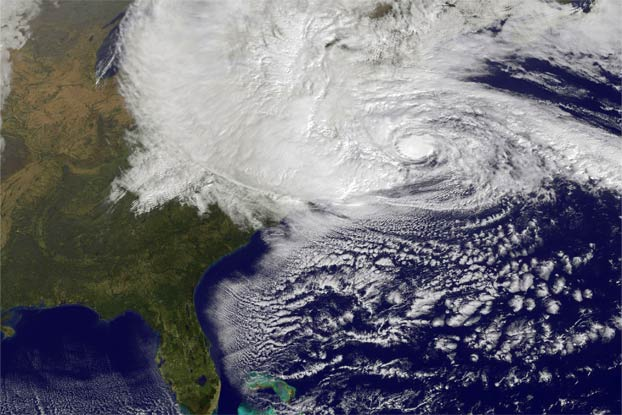
\includegraphics{../images/sandy-hurricane-1.jpg}
\caption{Hurricane Sandy, October 2012. Source:(NASA/GETTRY IMAGES).}
\end{figure}

Hurricanes have caused tremendous losses on the country's economy (\citet{Winkle2018}): they currently cost the government over \$28 billion each year. Besides the government, several industries are heavily impacted by hurricanes, including the insurance industry. For example, according to Bloomberg, hurricane Dorian caused the insurance industry losses of up \$25 billion, making it the most expensive natural disaster for the industry since 2017's Hurricane Maria (\citet{DSouza2019}). Therefore, the United States' Sustainable Development has identified economic losses from hurricane as a key indicator for the economic growth (\citet{SDG2018}). Disentangling the relative roles of variability and changes in Hurricane could contribute information useful to sustainable development goals.

Key frequently asked questions are: how climate affects hurricane, and what of the future hurricanes are more likely to be. To gain insight on these questions, we first have to look into historical records to discern the variability and changes of hurricanes, the analysis of which will help us to build predictive understanding of the influencing of climate on hurricane. Our working hypothesis is that: if greenhouse warming has caused a substantial increase in Atlantic hurricane activity, then the century scale increase in Atlantic hurricane since 1851 should have produced a long-term rise in measures of Atlantic hurricanes activity, similar to that seen for global temperature, for example. Therefore, we aim to dig into the original storm track file with more than 150 years of records of Atlantic tropical storm activities in order to examine variability and changes of Atlantic hurricane under global warming conditions. Specifically, three important questions we would like to address in this analysis are:

\emph{(1) What influences the change in category of hurricanes?}

\emph{(2) Has hurricane activity shifted north-ward?}

\emph{(3) Have humans already caused a detectable increase in Atlantic hurricane activity?}

\emph{(4) What other embedding patterns can we learn from the historical Atlantic hurricane record? How does this will help us to build predictive understanding of the influencing of climate on hurricane?}

\hypertarget{datasource}{%
\chapter{Data Source}\label{datasource}}

The storm track data presented in the analysis is downloaded from \href{https://www.nhc.noaa.gov/data/\#hurdat}{National Hurricane Center and Central Pacific Hurricane Center}, which is also known as the Atlantic hurricane database {[}HURDAT2: 1851-2018{]} (\url{https://www.nhc.noaa.gov/data/hurdat/hurdat2-1851-2018-120319.txt}) and the \href{https://www.aoml.noaa.gov/hrd/hurdat/comparison_table.html.}{HURDAT} data is downloaded from the {[}NOAA's Atlantic Oceanographic and Meteorological Laboratory{]} (\url{https://www.aoml.noaa.gov/}).

We choose to work with these data because they provide us with updated, complete and accurate information about hurricanes over the past 150 years (1851 - 2018). Since the Atlantic hurricane activity has shown very strong year-to-year and decade-to-decade variability, longer records or hurricanes are much needed.

In addition, we have also gathered the directly observed Atlantic Meridional Overturning Circulation (AMOC) index at 26 oN available for the period 27, 33 2004--2014, which is obtained from the {[}RAPID-WATCH MOC monitoring project{]} (www.rapid.ac.uk/rapidmoc). This is for the purpose of analyzing the linkage between hurricane frequency and climate variability, as well as the causes of the changes in Atlantic major hurricane frequency.

Furthermore, all the low-pass filtered data are obtained using the R function ``filtfilt'' with a Hamming window based low-pass filter at a 10-year cutoff period. One important thing to note about the names of hurricanes is that there are six names lists that have been used in rotation and re-cycled every six years. This means that there can be more than one hurricanes having the same name but happened in different years. We have tackled this problem by giving each hurricane a unique \texttt{storm-id}.

\hypertarget{datatrans}{%
\chapter{Data Transformation}\label{datatrans}}

The (\href{https://www.nhc.noaa.gov/data/hurdat/hurdat2-format-atlantic.pdf}{HURDAT2}) data has a comma-delimited, text format with six-hourly information on the location, maximum winds, central pressure, and (beginning in 2004) size of all known tropical cyclones and subtropical cyclones. The dataset is a combination of serveral subsets. Each subset is used for a storm track record which includes header information and values.
please refer to \href{https://www.nhc.noaa.gov/data/hurdat/hurdat2-format-atlantic.pdf}{this file} for detail information.

Firstly, we extract storm \texttt{id}, \texttt{name}, and \texttt{subtext\ length} from each subtext header, then read in data according to each \texttt{subtext\ length}, and merge data subset by indexing it with storm \texttt{id}, \texttt{name}. In the original text, you will find that the \texttt{name} is non-unique. Currently, there are six lists that are used in rotation and re-cycled every six years, i.e., the 2013 list is used again in 2019. For more information, please see tropical cyclone names. To avoid the future confusion, we create \texttt{storm-id} variable by combining \texttt{name} and \texttt{year} together (e.g., \emph{Sandy-2012}). In the original file, there are storms labeled with NAMEs but others labelled with \texttt{UNNAME}. Here, we use \texttt{name\_id} variable to indicate whether a storm has a name or not.

Secondly, we estimate \texttt{category} variable from wind speed based on \href{https://www.nhc.noaa.gov/aboutsshws.php}{Saffir-Simpson storm category}, calculate the diameter of the area experiencing hurricane strength winds (64 knots or above), \texttt{\_ts\_diameter\_} from extent of 34 kt wind radii maximum extent in northeastern quadrant (in nautical miles, \texttt{extent\_34\_NE}), 34 kt wind radii maximum extent in southeastern quadrant (in nautical miles, \texttt{extent\_34\_SW}), 34 kt wind radii maximum extent in northeastern quadrant (in nautical miles, \texttt{extent\_34\_NW}), and 34 kt wind radii maximum extent in southeastern quadrant (in nautical miles, \texttt{extent\_34\_SE}), \texttt{\_hu\_diameter\_} from extent of 64 kt wind radii maximum extent in northeastern quadrant - \texttt{extent\_64\_NE}, southeastern quadrant - \texttt{extent\_34\_SW}, northeastern quadrant, \texttt{extent\_64\_NW}), and southeastern quadrant - \texttt{extent\_64\_SE}.

Thirdly, we estimate the storm duration \texttt{tc\_dur\_track} to those with maximum sustained surface winds of at least 35 knot and defined storms and define \texttt{tc\_dur\_type} for type of the duration. Here, \texttt{S} indicates storms with duration of 2.0 days or less and will be mentioned in the following text as \emph{short-lived} storms, and \texttt{L} represnts storms with duration of more than 2.0 days and will be referred as ``medium-to-long lived'' storms.

Finally, the ocean surface temperature and the directly observed Atlantic Meridional Overturning Circulation (AMOC) index are \texttt{.nc} formate, we use \texttt{ncdf4} to read in data. Note that there is there is an ``ET'' typo in \emph{Status} of system in the \href{https://www.nhc.noaa.gov/data/hurdat/hurdat2-1851-2018-120319.txt}{HURDAT2}, which has been corrected to \texttt{EX} in the output \texttt{data\textbackslash{}clean\textbackslash{}hurricanes.csv} file.

\textbf{Meaning for each variables}

\texttt{\_id\_}

Storm id, which is unique. An id is a combination of 8 characters,

for example, `AL092011',

\begin{itemize}
\item
  AL (Spaces 1 and 2) -- Basin -- Atlantic
\item
  09 (Spaces 3 and 4) -- ATCF cyclone number for that year
\item
  2011 (Spaces 5-8, before first comma) -- Year
\end{itemize}

for detail information, please see \href{https://www.nhc.noaa.gov/data/hurdat/hurdat2-format-atlantic.pdf}{dataformat}

\texttt{\_name\_}

Storm Name, which is non-unique. There are six lists that are used in rotation and re-cycled every six years, i.e., the 2013 list is used again in 2019. For more information, please see \href{https://www.nhc.noaa.gov/aboutnames.shtml}{tropical cyclone names}.

\texttt{\_storm\_id\_}

Storm name and id combined, i.e., Sandy-2012

\texttt{\_unname\_label\_}

Storms have name or not (``yes'', ``no'')

\texttt{\_datetime,\ year,\ month,\ day,\ hour\_}

Date of report (in Universal Time Coordinate)

\texttt{\_record\_identifier\_}

C -- Closest approach to a coast, not followed by a landfall

G -- Genesis

I -- An intensity peak in terms of both pressure and wind

L -- Landfall (center of system crossing a coastline)

P -- Minimum in central pressure

R -- Provides additional detail on the intensity of the cyclone when rapid changes are underway

S -- Change of status of the system

T -- Provides additional detail on the track (position) of the cyclone

W -- Maximum sustained wind speed

\texttt{\_latitude,longitude\_}

Location of storm center

\texttt{\_status\_}

Storm classification (Tropical Depression, Tropical Storm, or Hurricane)

TD -- Tropical cyclone of tropical depression intensity (\textless{} 34 knots)

TS -- Tropical cyclone of tropical storm intensity (34-63 knots)

HU -- Tropical cyclone of hurricane intensity (\textgreater{} 64 knots)

EX -- Extratropical cyclone (of any intensity)

SD -- Subtropical cyclone of subtropical depression intensity (\textless{} 34 knots)

SS -- Subtropical cyclone of subtropical storm intensity (\textgreater{} 34 knots)

LO -- A low that is neither a tropical cyclone, a subtropical cyclone, nor an extratropical cyclone (of any intensity)

WV -- Tropical Wave (of any intensity)

DB -- Disturbance (of any intensity)

\texttt{\_category\_}

\href{https://www.nhc.noaa.gov/aboutsshws.php}{Saffir-Simpson storm category} (estimated from wind speed. -1 = Tropical Depression, 0 = Tropical Storm)

\texttt{\_max\_wind\_}

storm's maximum sustained wind speed (in knots)

\texttt{\_min\_pressure\_}

Air pressure at the storm's center (in millibars)

\texttt{\_ts\_diameter\_}

Diameter of the area experiencing tropical storm strength winds (34 knots or above)

\texttt{\_hu\_diameter\_}

Diameter of the area experiencing hurricane strength winds (64 knots or above)

\texttt{\_max\_category\_}

Maximum category of each storm track

\texttt{\_max\_status\_label\_}

Label (``TRUE'', ``FALSE'') to indicate whether the measurement is for the maximum status of each track

\texttt{\_max\_max\_wind\_}

The maximum value of the \texttt{max\_wind} for each track

\texttt{\_min\_min\_pressure\_}

The minimum value of the \texttt{min\_pressure} for each track

\texttt{\_max\_ts\_diameter\_}

The maximum value of the \texttt{ts\_diameter} for each track

\texttt{\_max\_hu\_diamter\_}

The maximum value of the \texttt{hu\_diameter} for each track

\hypertarget{missingval}{%
\chapter{Missing Values}\label{missingval}}

Here, we use \texttt{visna::extract} to look at the missing value patterns. \emph{The bars} beneath the columns in Figure \ref{fig:missingvalue-extracat-fig} show the proportions of missingness by variable, suggesting hurricane diameter \emph{(\texttt{hu\_diameter})} and storm diameter \emph{(\texttt{ts\_diameter})} both have the highest number of missing value and the columns suggest that they follow the same missing pattern, meaning when hurricane diameter is missing, storm diameter is also missing.

The third most missing variable is Pressure \emph{(\texttt{min\_pressure})} and \emph{the columns} show that Pressure is missing only when hurricane diameter and storm diameter are missing. The \emph{bars} on the right show the relative frequencies of the missing patterns, which suggest the most frequent missing patterns are in the combination of hurricane diameter, storm diameter and pressure, followed by the combination of hurricane diameter and storm diameter. Non-missing data are in the third meaning most of rows are completeness.

Finally, hurricane diameter and storm diameter are the most missing values because they are calculated from \emph{Wind Raddii} but \emph{Wind Raddii} values were not used before 2004.

\begin{figure}

{\centering 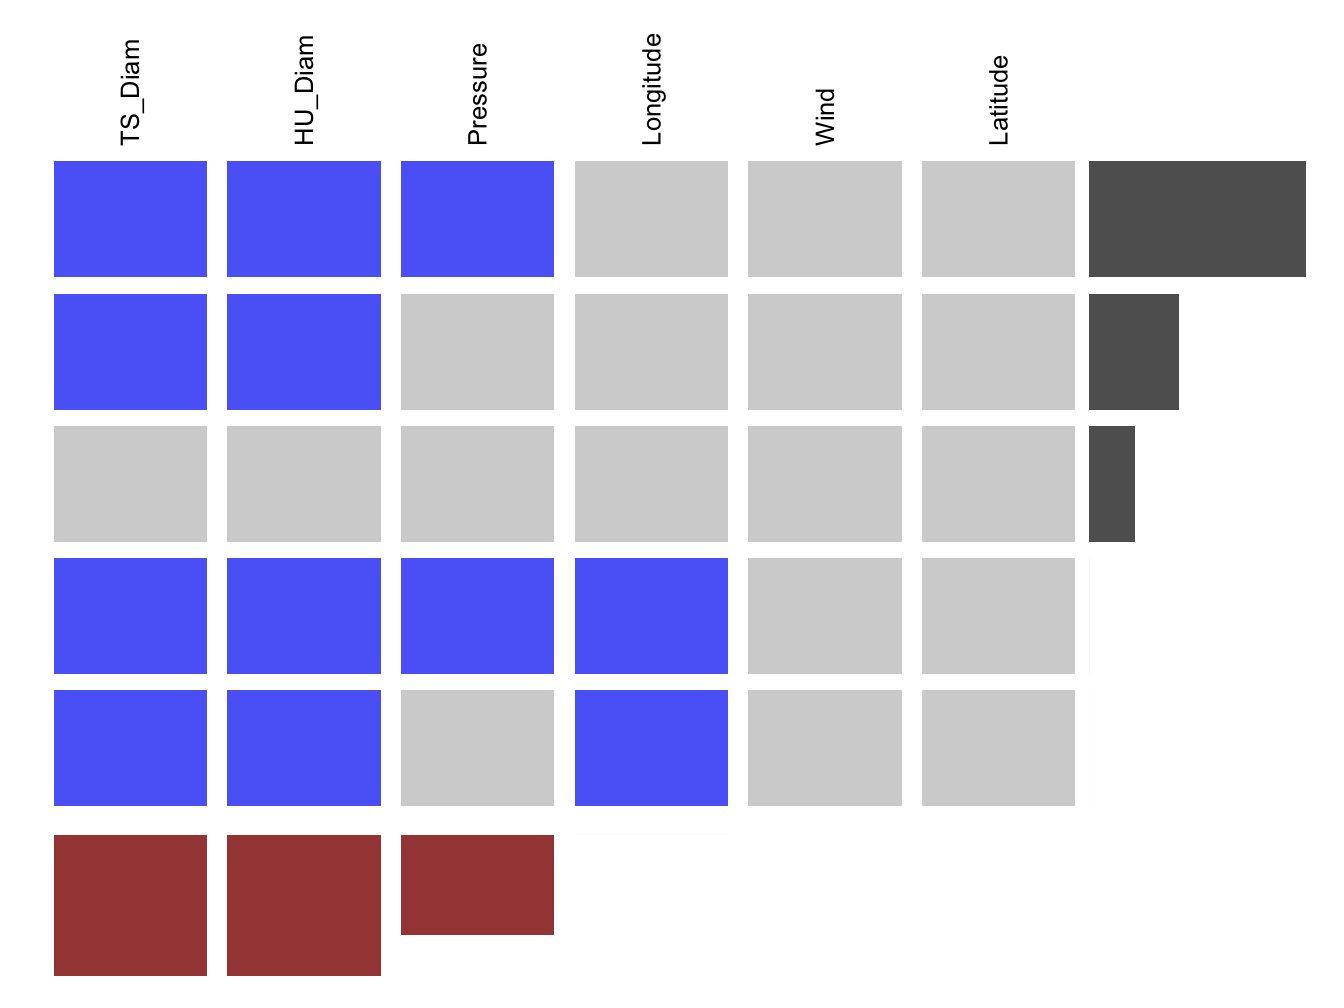
\includegraphics[width=0.8\linewidth]{edav-final-project_files/figure-latex/missingvalue-extracat-fig-1} 

}

\caption{Missing Values Patterns}\label{fig:missingvalue-extracat-fig}
\end{figure}

It is worth noting that almost all Pressure data are missing from 1850s to 1940s. The number of missing data is then decreasing from the 1940s, and there are no missing Pressure starting the 2000s (see Figure \ref{fig:missingvalue-pressure-year-fig}). The reasons for this are are the following: (1) in the early years, information about pressure was recorded by ships; those were few in numbers and thus a lot of pressure data could not be recorded (2) in more recent years, it became a common habit to replace missing pressure values by an analytical product such as sattelite data; (3) improvements in modern tools and technologies have provided us with a more powerful observation network than that in the early years.

\begin{figure}

{\centering 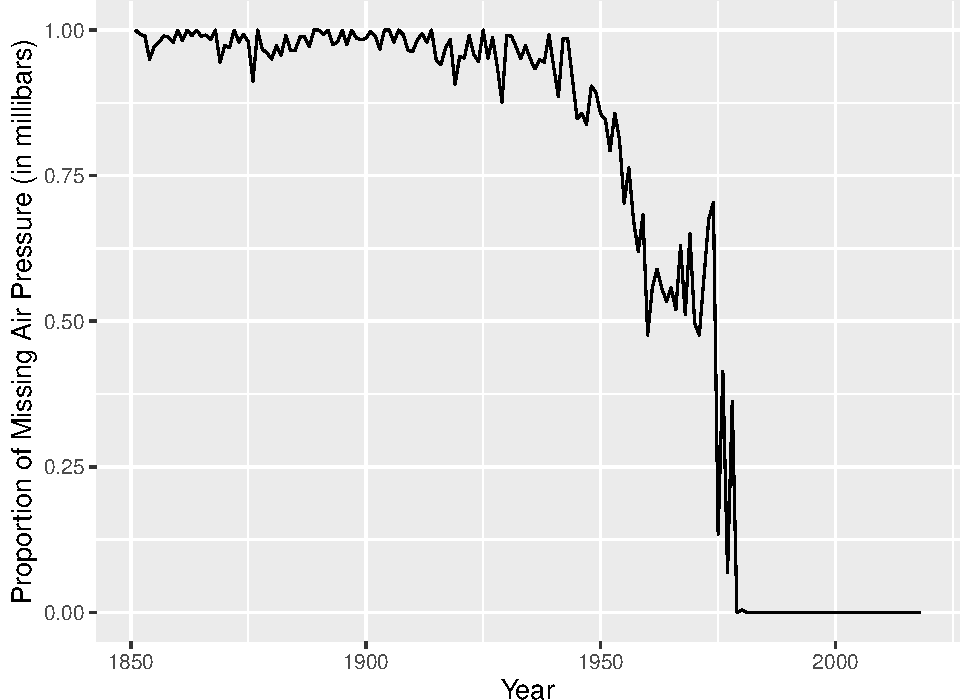
\includegraphics[width=0.8\linewidth]{edav-final-project_files/figure-latex/missingvalue-pressure-year-fig-1} 

}

\caption{Proportion of Missing Air Pressure at the Storm's Center By Year}\label{fig:missingvalue-pressure-year-fig}
\end{figure}

Another noticeable pattern in missing value relates to the name of tropical cyclones (see Figure \ref{fig:atlatnic-storms-unnamed-year-fig}).

Before the 1950s, it was not common practice to name tropical cyclones. This explains why we cannot find any cyclone with a name before that time. A couple were still not named after that, and the reason can be linked to the category: those cyclones are of category 0 and 1 (more information about categories can be found in part 5), which means that they could have been overlooked and therefore didn't receive any name.

\begin{figure}

{\centering 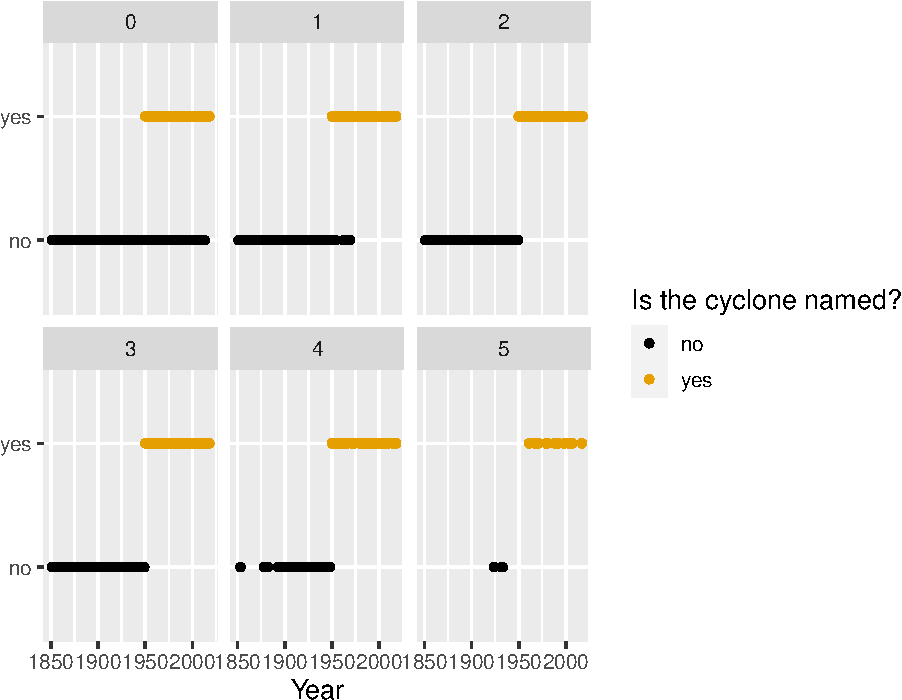
\includegraphics[width=0.8\linewidth]{edav-final-project_files/figure-latex/atlatnic-storms-unnamed-year-fig-1} 

}

\caption{Cyclones received names starting 1950s}\label{fig:atlatnic-storms-unnamed-year-fig}
\end{figure}

\hypertarget{result}{%
\chapter{Results}\label{result}}

\hypertarget{what-influences-the-change-in-category-of-a-hurricane}{%
\section{What influences the change in category of a hurricane?}\label{what-influences-the-change-in-category-of-a-hurricane}}

Hurricanes are classified in different categories based on the \href{https://www.nhc.noaa.gov/aboutsshws.php}{Saffir-Simpson} Hurricane Wind Scale, which classifies hurricanes with regards to their wind speeds and estimates potential property damages. The hurricanes categories come under five items:

\begin{enumerate}
\def\labelenumi{(\arabic{enumi})}
\tightlist
\item
  Category 1:
\end{enumerate}

Very dangerous winds from 64 to 82 knot (kt) that will lead to some damage such as roof damage or snapped tree branches. A famous hurricane of category 1 is \href{https://en.wikipedia.org/wiki/Hurricane_Danny_(1985)}{Danny}, which hit Cuba and the Gulf of Mexico in 1985.

\begin{enumerate}
\def\labelenumi{(\arabic{enumi})}
\setcounter{enumi}{1}
\tightlist
\item
  Category 2:
\end{enumerate}

Extremely dangerous winds from 83 to 95 kt that will produce extensive damage such as roof damage and siding, many toppled shallowly rooted trees and near-total power outage. A famous hurricane of category 2 is \href{https://en.wikipedia.org/wiki/Hurricane_Erin_(1995)}{Erin} which hit Florida in 1995 and caused 5 people to die and cost \$700 million (1995 USD).

\begin{enumerate}
\def\labelenumi{(\arabic{enumi})}
\setcounter{enumi}{2}
\tightlist
\item
  Category 3:
\end{enumerate}

Extremely dangerous winds from 96 to 112 kt will cause devastating damage such as removal of roof decking, power outage and power outage for days to weeks after the storm passes. \href{https://en.wikipedia.org/wiki/Hurricane_Katrina}{Katrina} is a famous hurricane of category 3 that lead to 1,836 deaths and \$81 billion (2005 USD) in property damage in 2005. Major states impacted were Louisiana and Mississippi.

\begin{enumerate}
\def\labelenumi{(\arabic{enumi})}
\setcounter{enumi}{3}
\tightlist
\item
  Category 4:
\end{enumerate}

Extremely dangerous winds from 113 to 136 kt that will cause catastrophic damage such as loss of most of the roof structure and exterior walls, fallen trees and power outage for weeks to months. A famous hurricane of category 4 is \href{https://en.wikipedia.org/wiki/Hurricane_Harvey}{Harvey} which hit Texas and Louisiana in 2017 with damage estimated to \$125 billion (2017 USD) and 107 deaths in the United States.

\begin{enumerate}
\def\labelenumi{(\arabic{enumi})}
\setcounter{enumi}{4}
\tightlist
\item
  Category 5:
\end{enumerate}

Extremely dangerous winds of 137 kt or higher that will cause catastrophic damage such as total roof and wall collapse, fallen trees, power outage for weeks to months and uninhabitable regions for weeks or months. A famous hurricane of category 5 is \href{https://en.wikipedia.org/wiki/Hurricane_Andrew}{Andrew}, which hit Louisiana and Florida in 1992 and whose damage accounts for \$41.5 billion (2011 USD) and 54 deaths (approximately 1 million people were evacuated before the storm).

Besides, it is also worth distinguishing hurricanes from tropical storms, whose maximum sustained surface winds range from 34 to 63 kt. They are labeled category 0 in our dataset.

The strength of a hurricane can also be assessed by its barometric pressure, that is the pressure at its center: the lower the barometric pressure, the stronger the hurricane.

Finally, the size of a hurricane is defined by its diameter.

Let's now examine those features on a parallel coordinate plot and see how they relate to each other.

\begin{figure}

{\centering 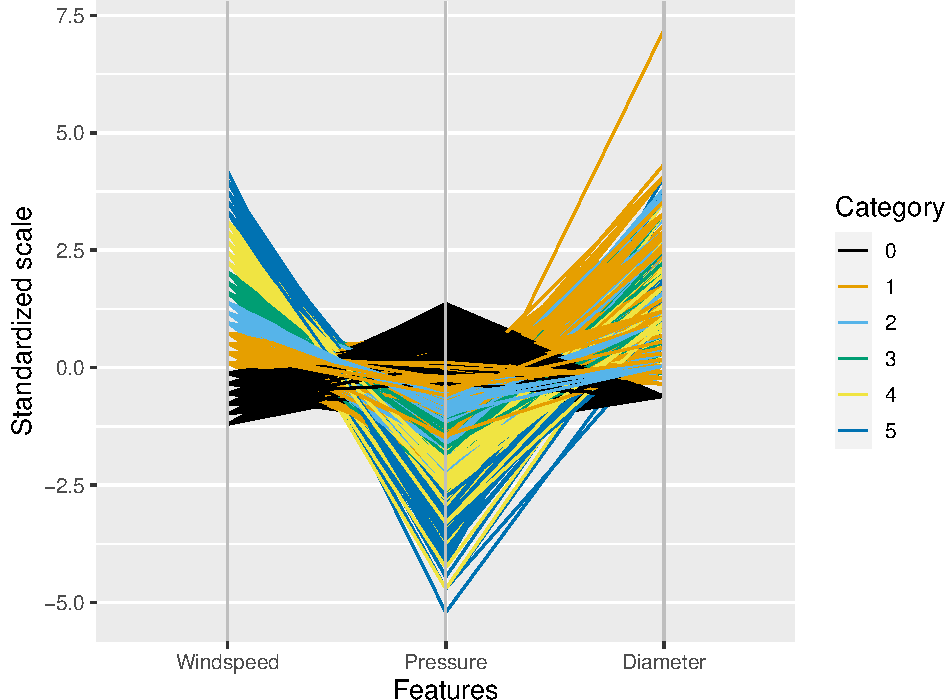
\includegraphics[width=0.8\linewidth]{edav-final-project_files/figure-latex/pcp-category-wind-pressure-fig-1} 

}

\caption{Windspeed and Pressure are indicators of cyclone category}\label{fig:pcp-category-wind-pressure-fig}
\end{figure}

First of all, as showing in Figure \ref{fig:pcp-category-wind-pressure-fig}, categories are clearly distinct in terms of windspeed and increase proportionally to this feature. This is consistent with the definition of the \href{https://www.nhc.noaa.gov/aboutsshws.php}{Saffir-Simpson Scale}. The same conclusion can be drawn for the \href{https://sciencing.com/barometric-pressure-hurricanes-22734.html}{barometric pressure measured at the center of the hurricane}: for low pressures, the hurricane will be overall of a higher category. The distinction is however not as clear as for windspeed and some overlap can be noticed.

Furthermore, no relationship can be established between the diameter of the area experiencing hurricane strength winds of 64 knots or above hurricane diameter \emph{(\texttt{hu\_diameter})}, which would mean that the category, wind speed and min pressure will not determine the potential areas that will be affected by hurricane.

Note that all tropical storm have a diameter equal to 0: this is because the variable used for the graph is hurricane diameter, which accounts for the diameter of hurricanes. The diameter of the area experiencing tropical storm strength winds (34 knots or above) is reported in a separated variable called storm diameter \emph{(\texttt{ts\_diameter})}. As this project focuses on hurricanes, and these two parameters are highly correlated to each other, the decision was made to not include it in the graph.

\hypertarget{a-first-look-into-the-evolution-of-the-category-of-hurricanes}{%
\subsection{A first look into the evolution of the category of hurricanes}\label{a-first-look-into-the-evolution-of-the-category-of-hurricanes}}

Let's now check whether a hurricane sticks to one category in its lifetime or if it changes overtime. To do so, we select three hurricanes of the same year: Irma (Florida), Maria (North Carolina) and Gert (North of Atlantic Ocean), which all occurred in 2017.

\begin{figure}

{\centering 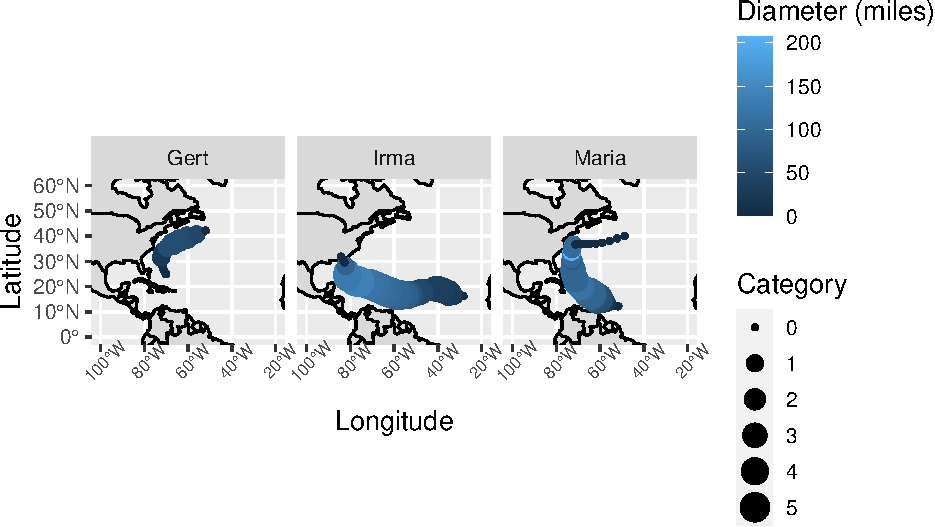
\includegraphics[width=1\linewidth]{edav-final-project_files/figure-latex/each-track-develop-fig-1} 

}

\caption{Three Example Hurricanes in 2017}\label{fig:each-track-develop-fig}
\end{figure}

From Figure \ref{fig:each-track-develop-fig}, it can be noted that both Irma and Maria grew in intensity to reach category 5, while Gert \textbf{only} reached category 2 as a maximum. A difference in lifetime can also be highlighted (almost 2 weeks vs a couple days). As both Irma and Maria hit Southern states and Gert occured at a Northern location, the following hypothesis is stated: is the maximum category reached by a hurricane dependent on its location? That is, \emph{is there a difference between the maximum category reached by Southern and Northern hurricanes?}

\begin{figure}

{\centering 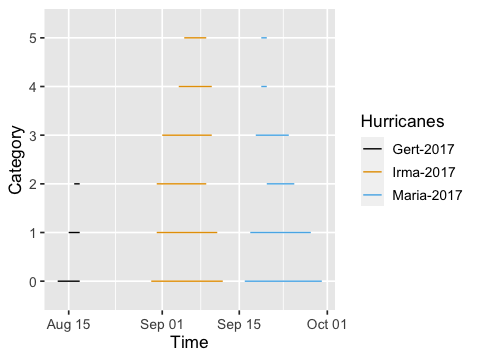
\includegraphics[width=0.8\linewidth]{edav-final-project_files/figure-latex/each-track-develop-time-fig-1} 

}

\caption{Time Series of Three Example Hurricanes in 2017}\label{fig:each-track-develop-time-fig}
\end{figure}

Before testing that hypothesis, it is worthy to note that the vertical jumping lines in the time series of hurricanes (Figure \ref{fig:each-track-develop-time-fig}). These suggest that hurricanes are highly dynamic and can lose/gain energy in only a couple hours. This concept is illustrated by the following time series (Figure \ref{fig:tc-dramatic-fig}), showing a close up of hurricane Irma evolution on September 9th 2017; in a couple hours, the hurricane when from category 5 to category 2.

\begin{figure}

{\centering 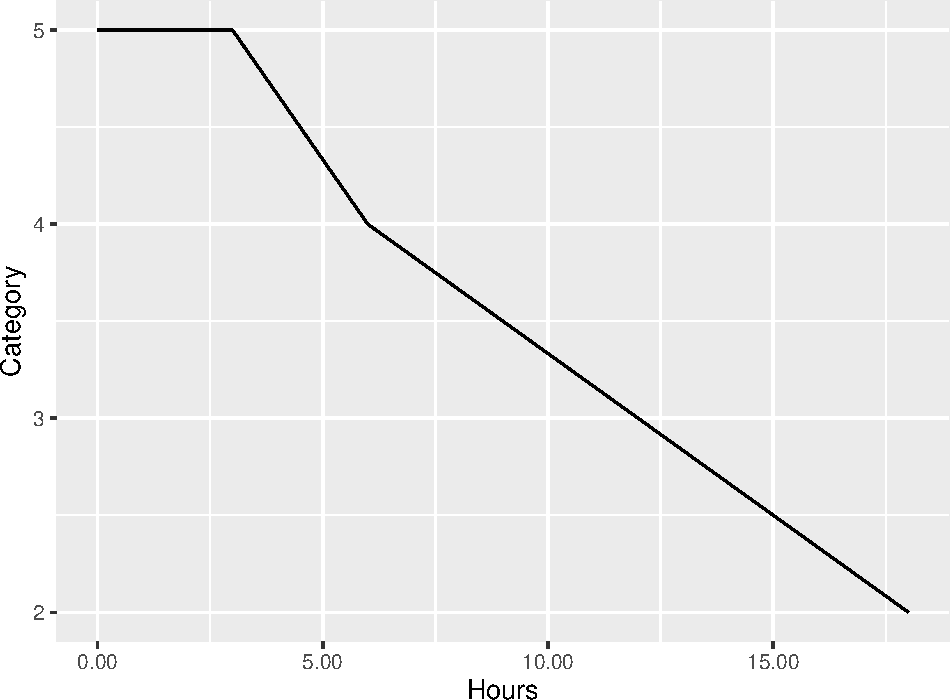
\includegraphics[width=0.8\linewidth]{edav-final-project_files/figure-latex/tc-dramatic-fig-1} 

}

\caption{Close Up of Time Series of Hurricane Irma in 2017}\label{fig:tc-dramatic-fig}
\end{figure}

\hypertarget{is-there-a-difference-between-the-maximum-category-reached-by-southern-and-northern-hurricanes}{%
\subsection{Is there a difference between the maximum category reached by Southern and Northern hurricanes?}\label{is-there-a-difference-between-the-maximum-category-reached-by-southern-and-northern-hurricanes}}

Let's now verify whether the hypothesis holds. The Figure \ref{fig:each-track-develop-fig} depicts the path of each hurricane across time and also colors the diameter the area experiencing hurricane strength winds of 64 knots or above and sized according their categories.

Each hurricane formed in the low latitude east with a low category, then intensified (large circle and bluer) as it extracted energy from the warm/moist air over the oceans. As a result, its category evolved with time until it reached a certain point then dissipated. The hurricanes then broke apart because they move through cold water (e.g, Maria) or move over land (e.g., Irma) which made them losing touch with the hot water that powered them.

When hurricanes start at different location point, they absorb different amount of energy throughout their progression towards the west or northwest. This will lead to different energy formation that will determine the highest wind level measured, and in turn decide what that category of that hurricane will be.

The comparison of the hurricane track and intensity indicates that the longer the hurricane stay over the southern warm water, the stronger it gets to be (see Irma), while the northern formed storms, like Gert, could not reach high category and they die out a few hours after they start because they do not have enough energy to become a hurricane.

This seems to confirm the hypothesis stated above: there seems to be an interesting relationship between location and category of a hurricane. In addition, hurricanes seem to reach higher categories when located in the South of the Atlantic Ocean than in the North.

\begin{figure}

{\centering 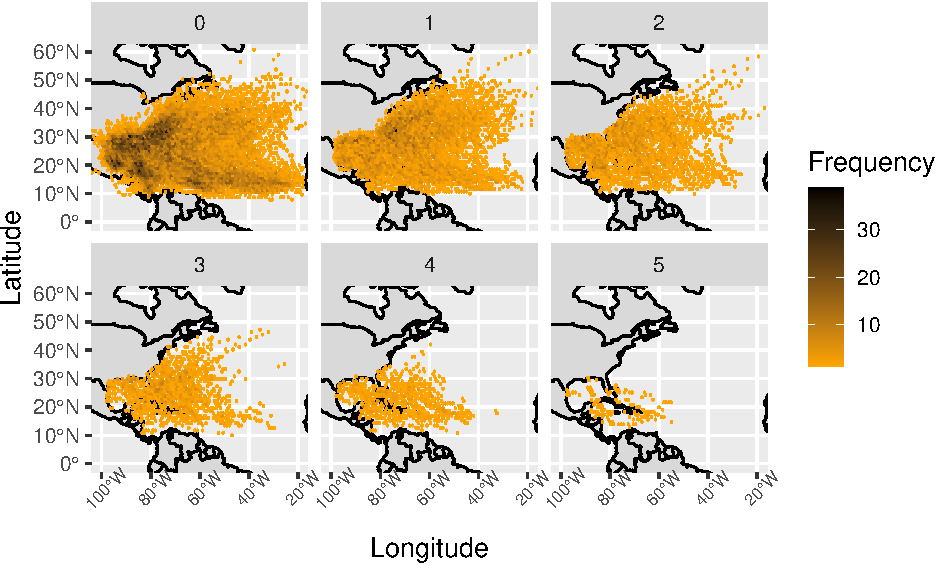
\includegraphics[width=0.8\linewidth]{edav-final-project_files/figure-latex/co2-year-fig-1} 

}

\caption{Frequency of Hurricanes across the United States}\label{fig:co2-year-fig}
\end{figure}

Let's now check whether the hypothesis can be extended in terms of frequency. The frequency of hurricane by location for each category. Figure \ref{fig:co2-year-fig} shows that storms and hurricanes disappear when they reach the land or the northern water.

The low category storms (e.g., category 0 and 1) with the highest density along the coastline can reach further North, while the high category hurricanes (4 and 5) only appear in the South. The highest density along the coastline is related to the progress of the small tropical depressions. When these small depressions travel over the ocean to the US eastern coast, they gain energy and update to the category 0 storm. It is worth to note that as category increases, their north boundary seems to shift toward the south, suggesting the feature of storms and hurricanes are location-related.

We build a Shiny Web Application for the Interactive Component in order to assist with visualizing this result.

\hypertarget{does-hurricane-activity-shift-north-ward}{%
\section{Does hurricane activity shift north-ward?}\label{does-hurricane-activity-shift-north-ward}}

Next, we want to assess whether hurricane activity is shifting North. A recent study showed that the locations of tropical cyclones is shifting poleward (i.e.~north-ward) globally (\href{https://www.climatecentral.org/news/warming-may-shift-hurricane-impacts-17437}{Thompson}). If true, this implies heavy consequences for the Northern part of the United States. Southern states such as Florida have already taken steps to improve its approach to hurricanes, such as property structure improvements, rescue boats and vehicles investments, and emergency workers trainings; if the frequency of tropical cyclones is indeed shifting North, Northern states should consider taking similar actions.

Before exploring the above hypothesis, it is worth redefining latitude and longitude:

\textbf{Latitude} is the measurement of a place on Earth with regards to its distance north or south-wise from the Earth's equator. Latitude is expressed in degrees followed by the letter N or S whether the location measured is North or South from the equator. Interesting examples for this project are Miami's latitude (\textasciitilde{}26°N) and New York City's latitude (\textasciitilde{}41°N).

\textbf{Longitude} is the measurement of a place on Earth with regards to its distance west or east-wise from the meridian at Greenwich, England. It is also measured in degrees and followed by the letter W or E depending on whether the location of interest is West or East from the meridian.

We will focus on latitude to verify whether hurricane activity seems to be changing directions.

\begin{figure}

{\centering 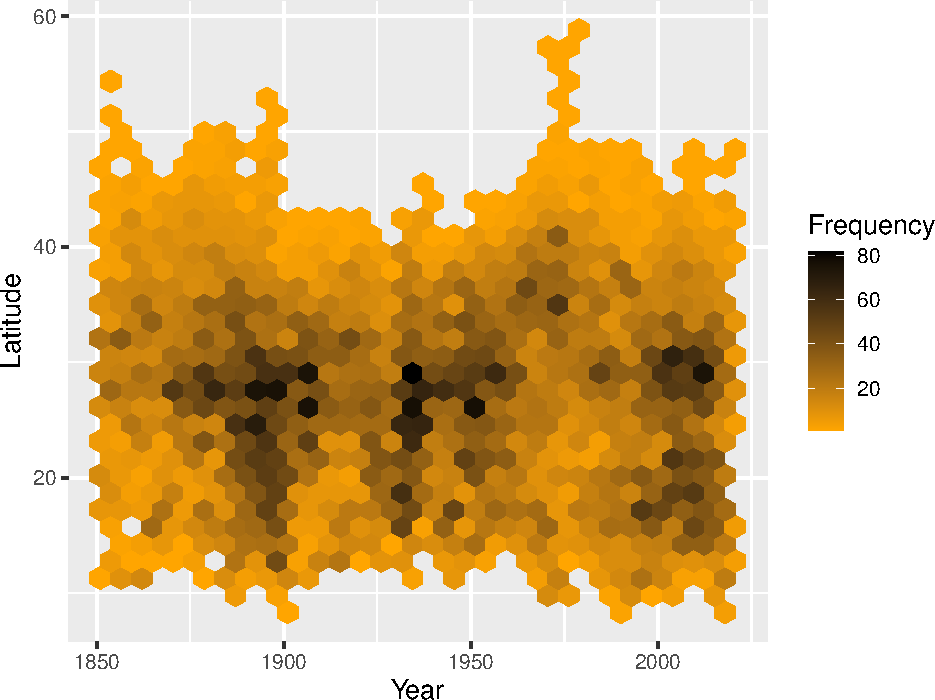
\includegraphics[width=0.8\linewidth]{edav-final-project_files/figure-latex/hurricane-north-fig-1} 

}

\caption{Frequency of Hurricanes by Latitude over Years}\label{fig:hurricane-north-fig}
\end{figure}

Figure \ref{fig:hurricane-north-fig} shows a heatmap of hurricane activity based on time and location.

While tropical cyclones frequency seems to be consistently higher at lower latitudes, one can observe an increase in cyclones activity at higher latitudes in the 1970s. However, this shift does not seem to be permanent as the frequency of tropical cyclones seems to decrease again in the following decades.

Besides, if we look at the tropical cyclones activity faceted on category (Figure \ref{fig:hurricane-north-category-fig}), the shift in location seems to be focused on tropical storms (category 0) and hurricanes of category 1. Hurricanes of category 4 are also more frequent on higher latitudes in the 1970s but the frequency remains at a low level and the activity returns to lower latitudes in the following decades. These observed trends would therefore not justify investments in hurricane-proofed facilities for Northern States.

\begin{figure}

{\centering 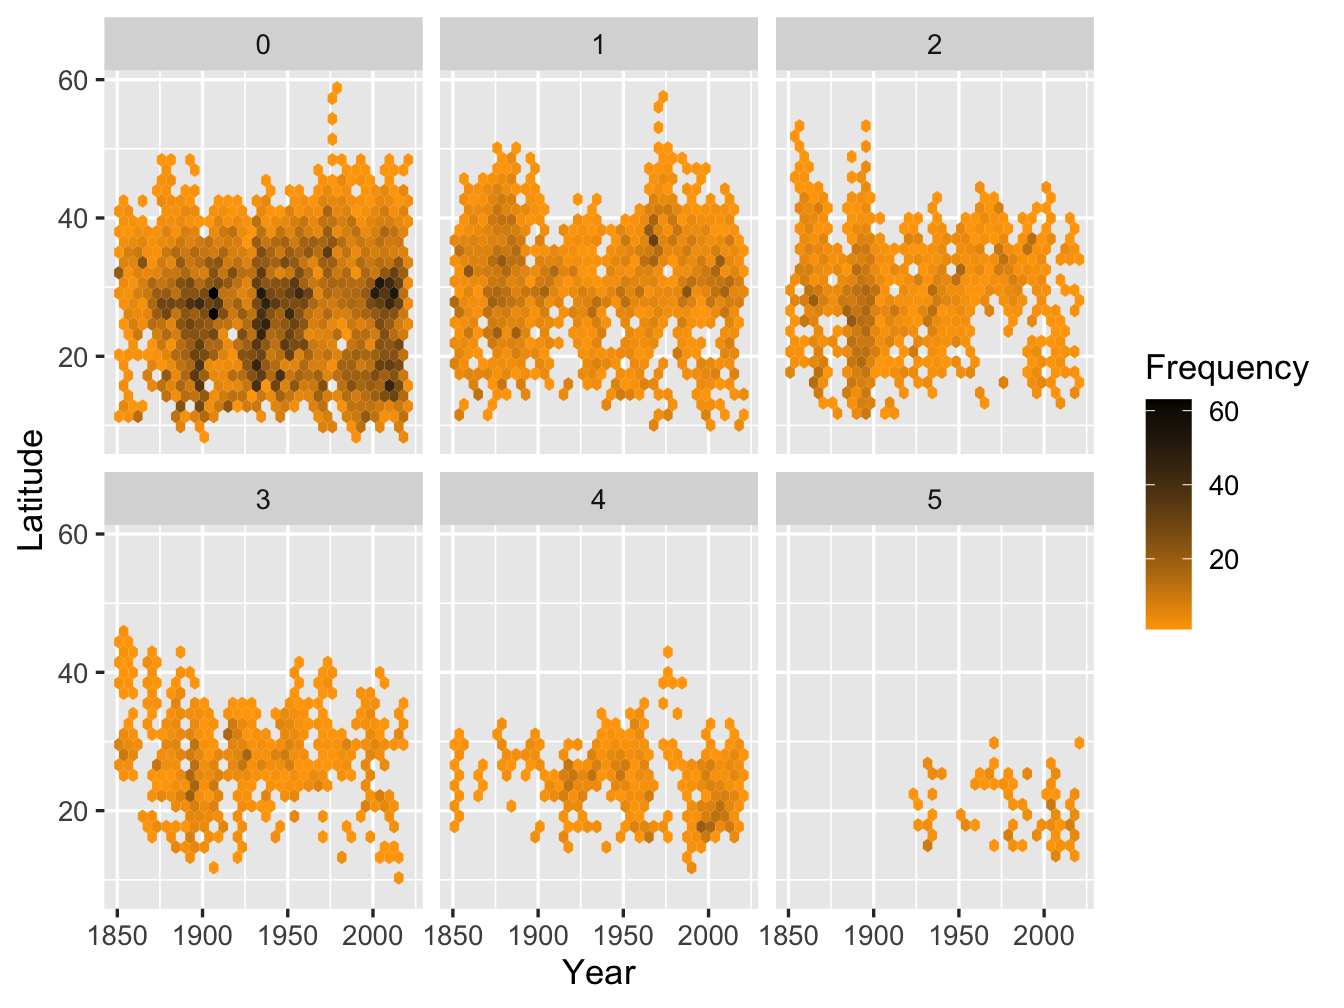
\includegraphics[width=0.8\linewidth]{edav-final-project_files/figure-latex/hurricane-north-category-fig-1} 

}

\caption{Frequency of each Hurricane Category over Years}\label{fig:hurricane-north-category-fig}
\end{figure}

\hypertarget{have-humans-already-caused-a-detectable-long-term-increase-in-atlantic-hurricane-activity}{%
\section{Have humans already caused a detectable long-term increase in Atlantic hurricane activity?}\label{have-humans-already-caused-a-detectable-long-term-increase-in-atlantic-hurricane-activity}}

As we can see from Figure \ref{fig:ts-co2-year-fig}, the global CO2 concentration has increased, and the tropical Atlantic sea surface temperature show significant warming trends (Figure \ref{fig:ts-sst-year-fig}).

\begin{figure}

{\centering 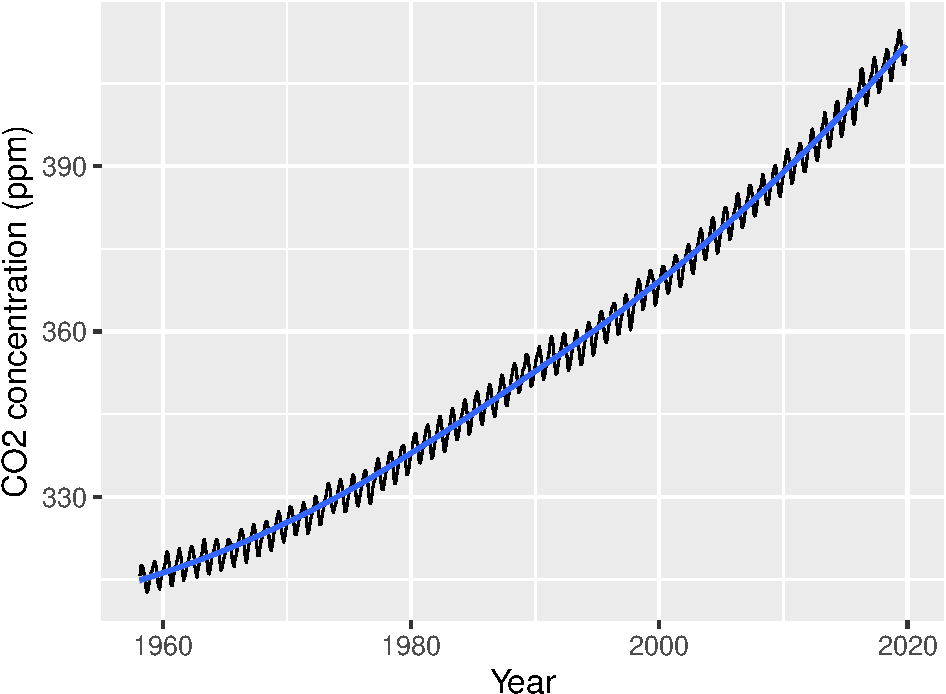
\includegraphics[width=0.8\linewidth]{edav-final-project_files/figure-latex/ts-co2-year-fig-1} 

}

\caption{Time Series of Atmospheric CO2 (ppm)}\label{fig:ts-co2-year-fig}
\end{figure}

\begin{figure}

{\centering 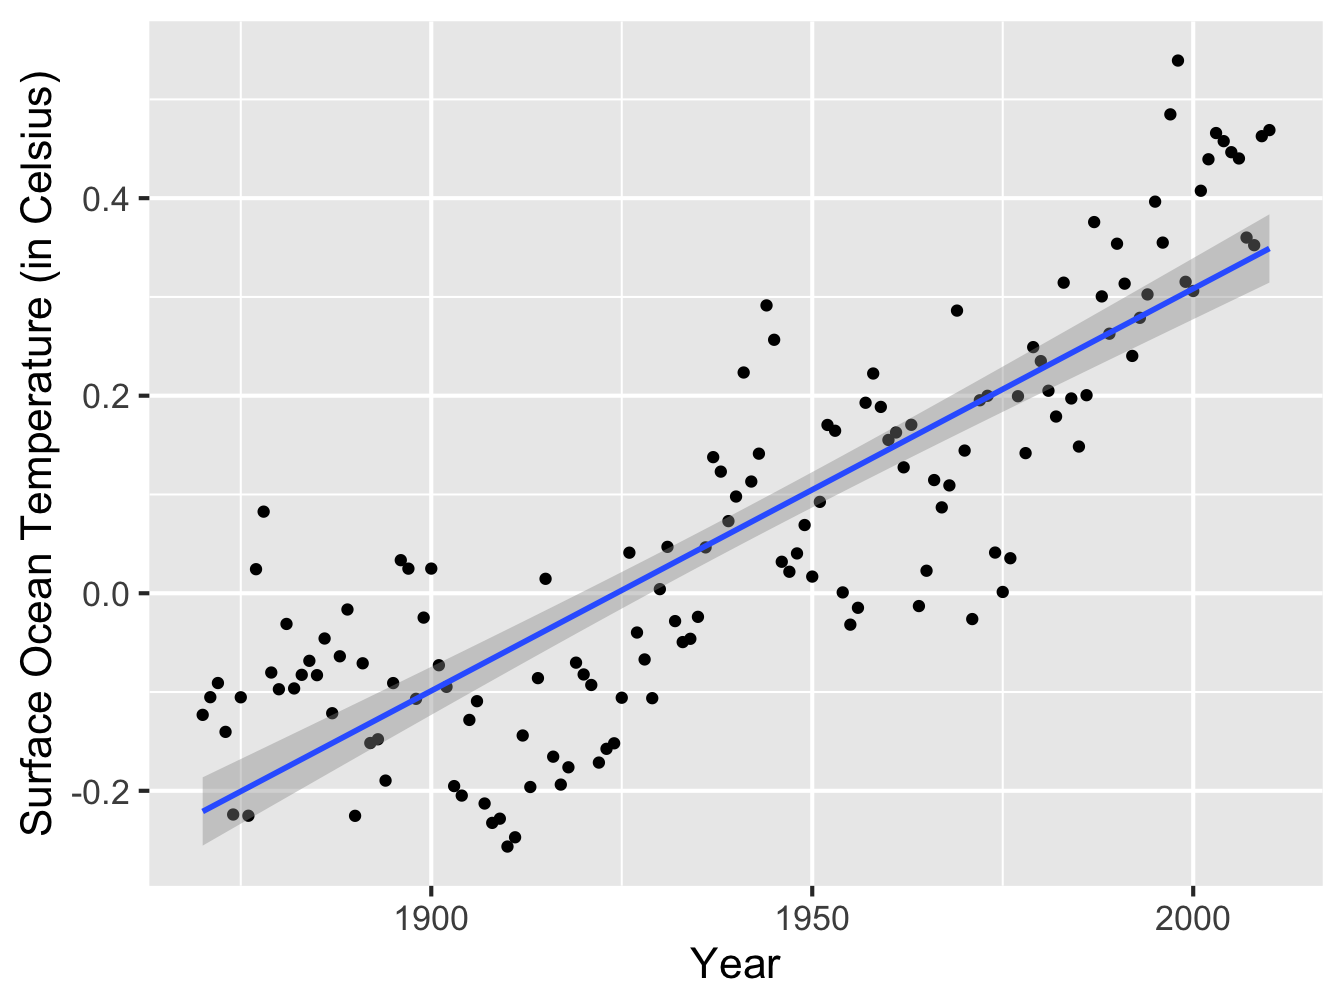
\includegraphics[width=0.8\linewidth]{edav-final-project_files/figure-latex/ts-sst-year-fig-1} 

}

\caption{Time Series of Ocean Surface Temperature}\label{fig:ts-sst-year-fig}
\end{figure}

Besides, one can also observed an increase in the number of storms and hurricanes in the Atlantic from 1851 to 2018 (Figure \ref{fig:ts-storm-year-fig}). We used this finding to ask the following question: \emph{is there a link between greenhouse-induced warming and changes in the Atlantic storms frequency (Figure \ref{fig:ts-storms-duration-year-fig})?}.

\begin{figure}

{\centering 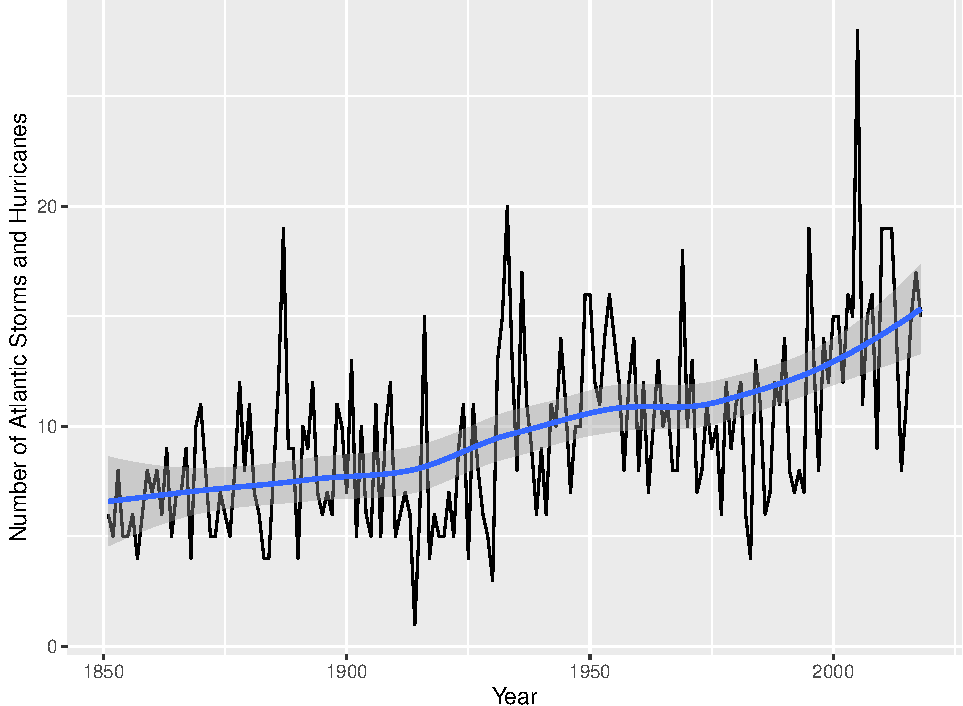
\includegraphics[width=0.8\linewidth]{edav-final-project_files/figure-latex/ts-storm-year-fig-1} 

}

\caption{Number of Atlantic Storms and Hurricanes Over Time}\label{fig:ts-storm-year-fig}
\end{figure}

Based on past Atlantic hurricanes records from 1878-2006, scientists concluded that the increasing trend in the number of Atlantic storms is almost completely due to the increase in short-duration storms (less than 2 days) (\citet{Landsea2010}), suggesting that only the count of short-duration storms follow a similar trend as the CO2 concentration and surface ocean temperature.

However, at the time, the focus was on storms that could have had an impact on ship traffic and, therefore, it is very likely that short-lived storms were overlooked in the earlier parts of the record. Besides, once our group explored the dataset with extra ten years' record, we found that there is an increase trend on both short-lived and long-lived storms.

\begin{figure}

{\centering 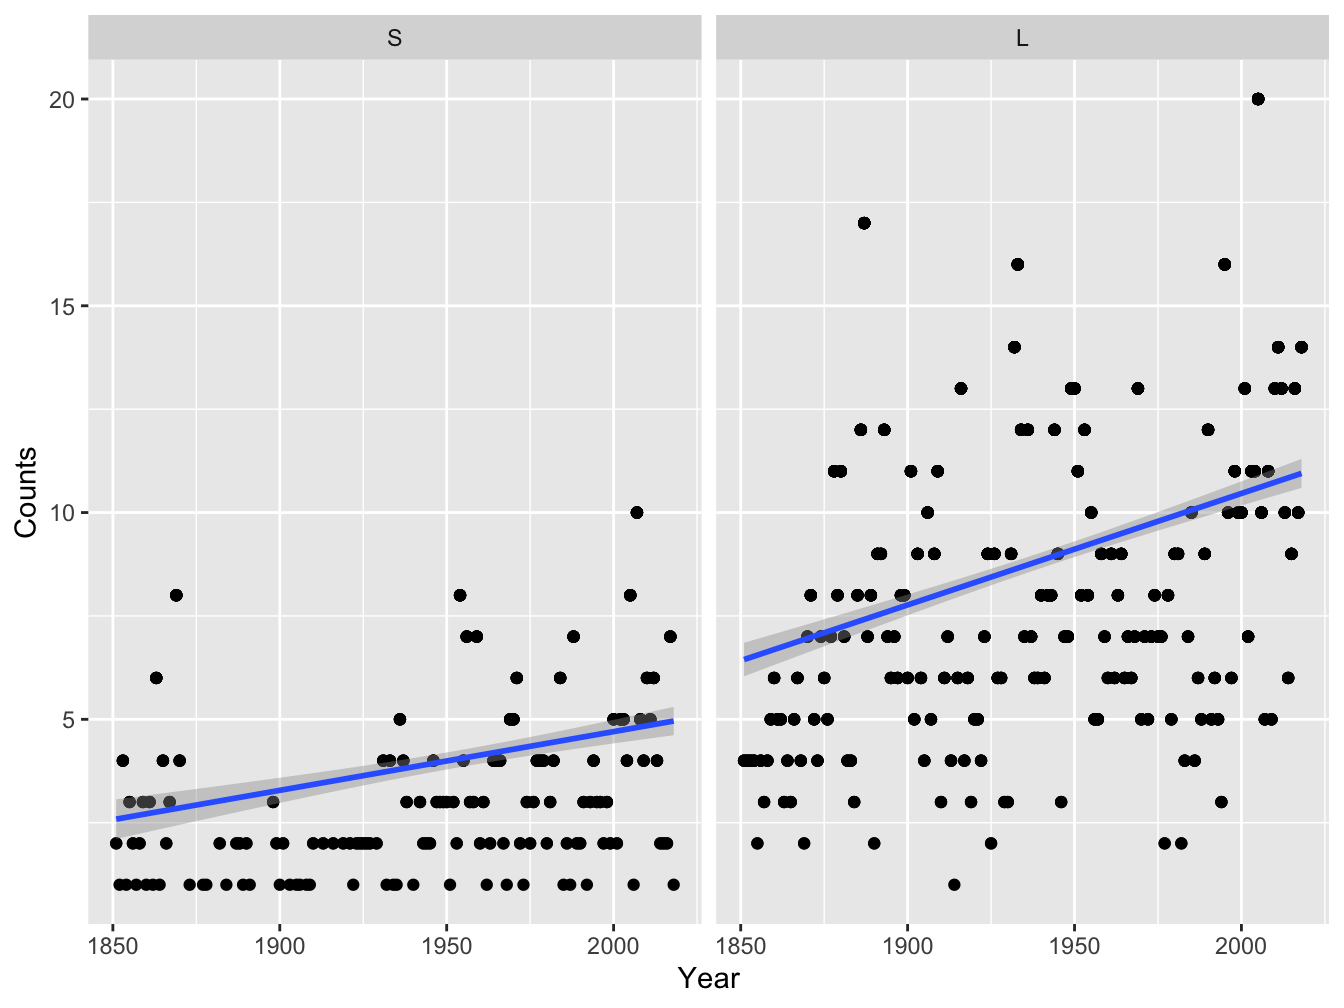
\includegraphics[width=0.8\linewidth]{edav-final-project_files/figure-latex/ts-storms-duration-year-fig-1} 

}

\caption{Time Series of Atlantic Short-lived (`S`) and Long-lived (`L`) Storms and Hurricanes Number}\label{fig:ts-storms-duration-year-fig}
\end{figure}

This means that the evolution of the number of cyclones over time follows a similar trend as the CO2 concentration and surface ocean temperature. This could mean that humans have had an impact on the increase of hurricane activity, but to prove that this is a causation and not only a correlation, deeper research and statistical tests should be performed.

```

\hypertarget{intercom}{%
\chapter{Interactive Component}\label{intercom}}

\begin{Shaded}
\begin{Highlighting}[]
\NormalTok{knitr}\OperatorTok{::}\KeywordTok{include_app}\NormalTok{(}\StringTok{'https://hurricane.shinyapps.io/01_01/'}\NormalTok{, }\DataTypeTok{height =} \StringTok{'600px'}\NormalTok{)}
\end{Highlighting}
\end{Shaded}

\begin{figure}

{\centering \href{https://hurricane.shinyapps.io/01_01/}{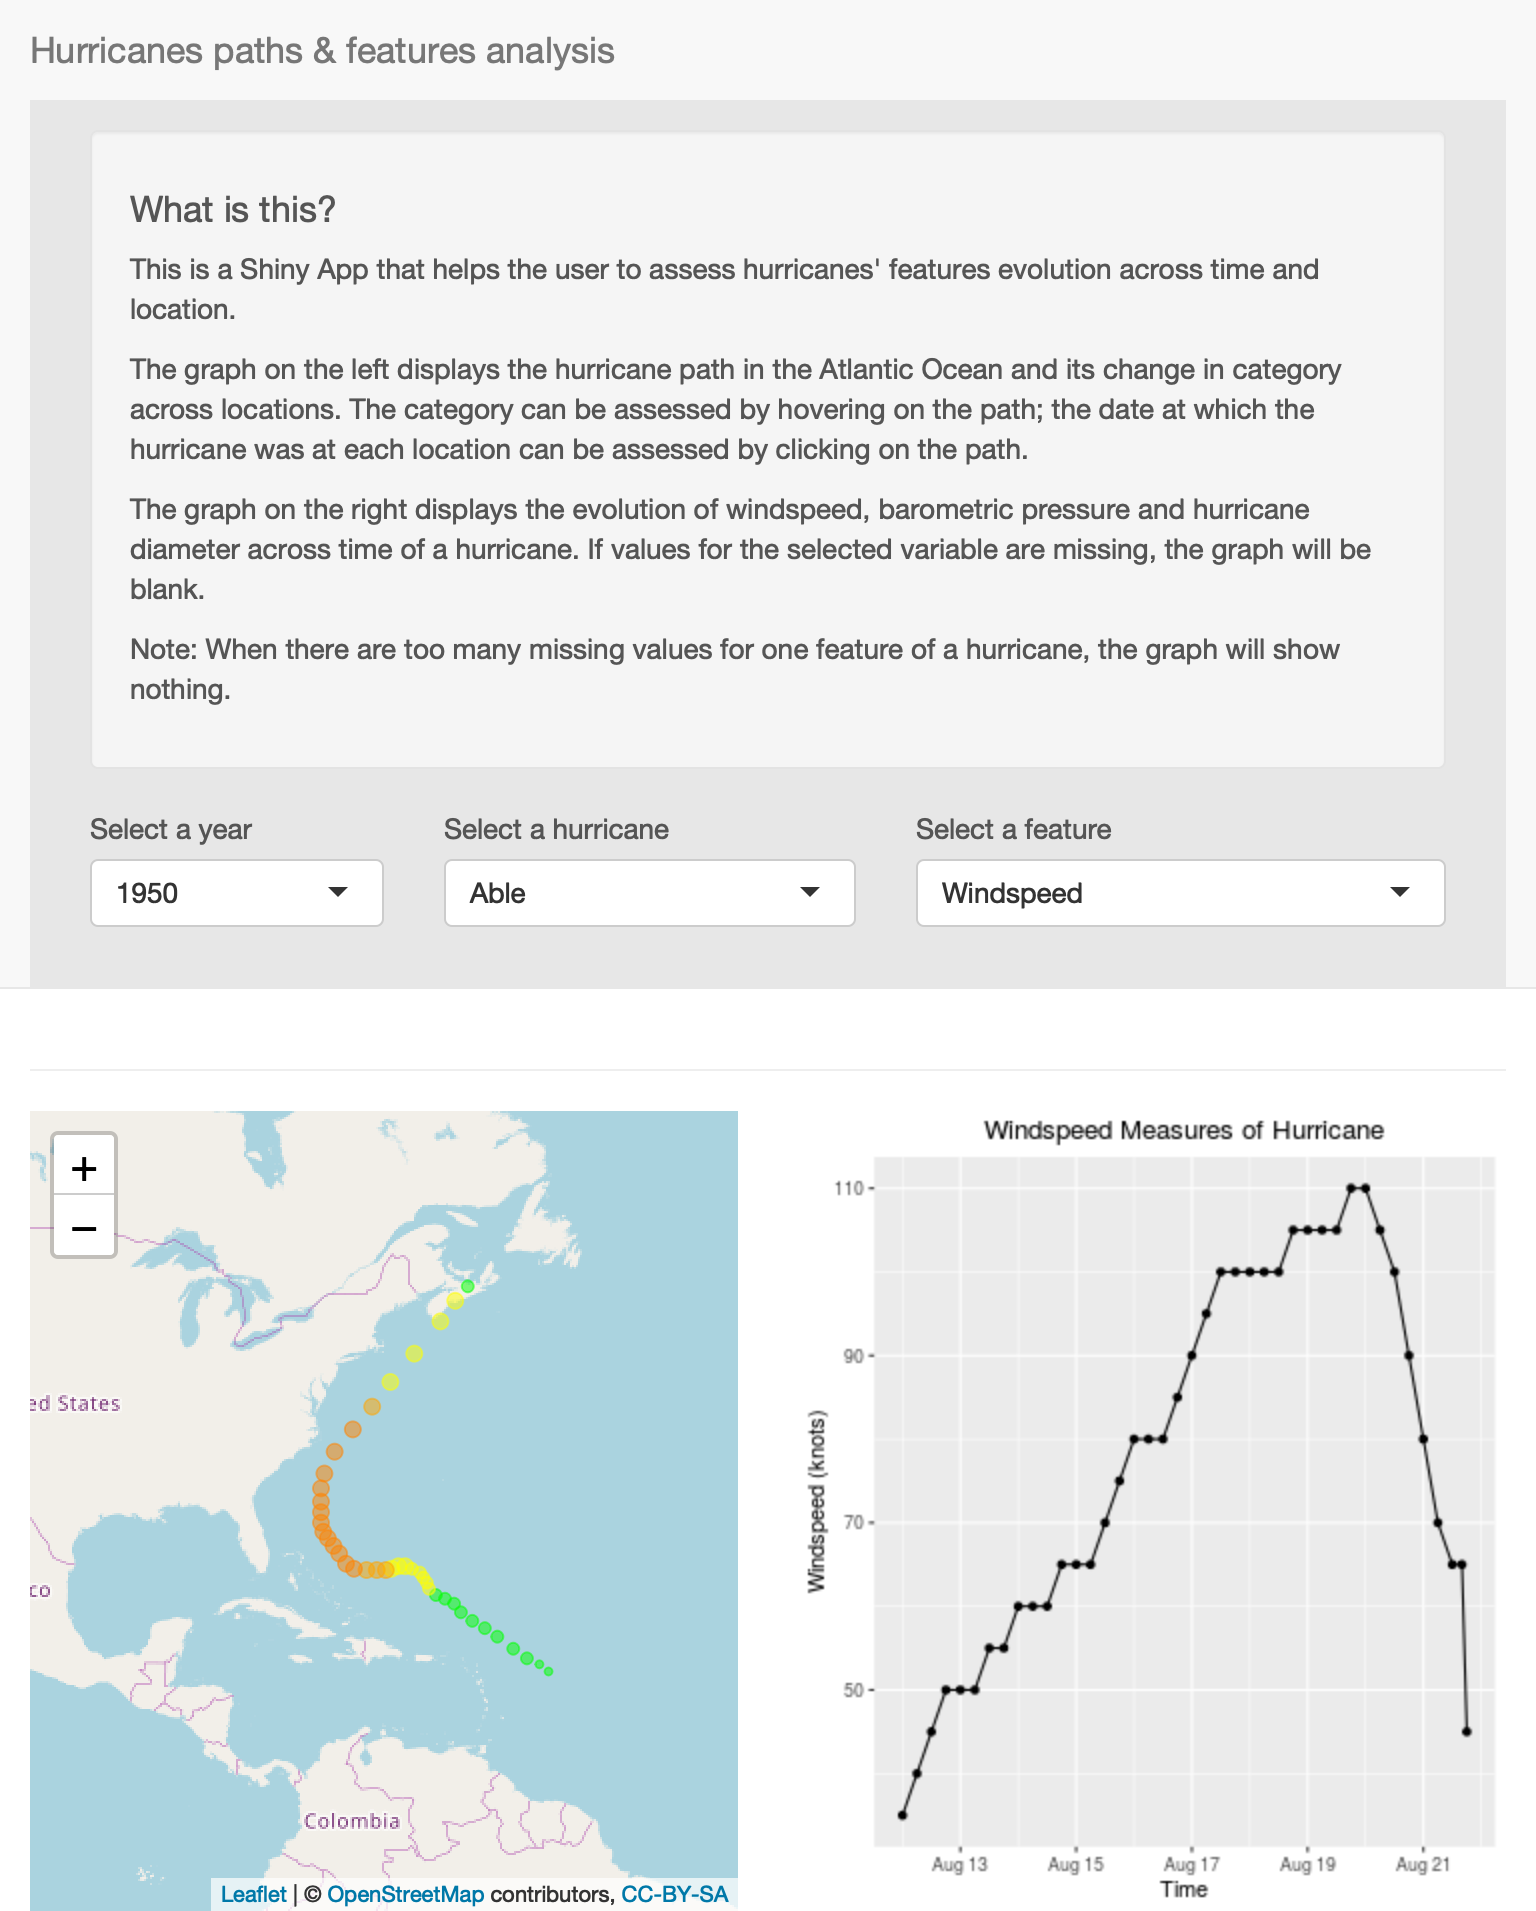
\includegraphics{edav-final-project_files/figure-latex/storm-track-1} }

}

\caption{app}\label{fig:storm-track}
\end{figure}

The following Shiny App that helps the user to assess hurricanes' features evolution across time and location as done in part 5.1 of this analysis.

The graph on the left displays the hurricane path in the Atlantic Ocean and its change in category across locations. The category can be assessed by hovering on the path; the date at which the hurricane was at each location can be assessed by clicking on the path.

The graph on the right displays the evolution of windspeed, barometric pressure and hurricane diameter across time of a hurricane. If values for the selected variable are missing, the graph will be blank.

If the server is too slow and the app doesn't appear on your screen, follow this \href{https://github.com/jqz300/edav_proj}{Github link} to download the necessary files and run the app locally.

\hypertarget{conclusion}{%
\chapter{Conclusion}\label{conclusion}}

In this analysis, we explore the century long storm records {[}HURDAT2: 1851-2018{]} (\url{https://www.nhc.noaa.gov/data/hurdat/hurdat2-1851-2018-120319.txt}) to investigate the characteristics of Atlantic storms and hurricanes and examine their changes under global warming conditions. The analysis results indicate that:

\begin{enumerate}
\def\labelenumi{(\arabic{enumi})}
\item
  The {[}Saffir-Simpson{]} scale (\url{https://www.nhc.noaa.gov/aboutsshws.php}) that is currently widely used to define category of hurricane reflects well the strength of wind and pressure. However, no relationship could be established between the category and size of the cyclones, indicating that a high category hurricane can be of small size and vice versa. Finally, Southern cyclones seem to reach a higher category than Northern cyclones in their lifetime, indicating a relationship between the category and the location. The century long Atlantic storms and hurricanes tracks and features can be easily visualized from \href{https://hurricane.shinyapps.io/shinyapp/}{storm shinyapp}.
\item
  While recent studies indicate a global North-ward shift in cyclones activity, we did not find strong evidence of this trend in our data. An increase of activity in the North was observed in the 1970s but seemed to decrease in the following decades. Besides, that shift seemed to be due to mostly an increase in frequency of cyclones of category 0 and 1, which are less worrying than cyclones of higher categories.
\item
  Human activities may have already caused the changes in the Atlantic storm and hurricane activity, reflected by the increasing number of the Atlantic cyclones. However, exploratory analysis can only help us identify similarity in trends and not confirm that one is the cause of the other. In order to do the latter, further research and statistical testing should be performed.
\end{enumerate}

\bibliography{proj.bib,packages.bib}


\end{document}
